\section{Methods}

\subsection{Data Preprocessing}
\subsubsection{Data Source \& Preprocessing}
To generate analyzable text this project utilizes an existing `.mobi' file of \infinitejest. This file is put through a .mobi to HTML conversion to generate an HTML formatted file as well as a .mobi to raw text conversion. This enables the use of regular expressions to find and parse various text features automatically. Thus the HTML text is used to identify endnote locations such that simplified endnote tags can be inserted into the raw text file. Similarly, regular expressions are used to indentify where section breaks exist according to the section annotations given by the book Elegant Complexity \cite{carlisle_2007}. The raw text is split on these sections and saved into separate files. Likewise each endnote is saved into a separate file. In each of these files, we remove all inessential special characters (e.g. special quotes). As we employ the Python 3.7 standard, all text files are imported as unicode.

\subsubsection{Named Entitiy Recognition}

A major challenge with \infinitejest is the abundant use of pseudonyms and aliases of the 200+ characters in the novel. As our network uses characters as nodes, identifying named entities and their synonym coreference resolutions (not for pronouns) requires an extensive hand-engineered approach. We utilize the Named Entity Recognition (NER) parser of the Python library SpaCy \cite{spacy2} augmented with its own Matcher parser. By running the existing NER model on the text, we compare candidate entities generated from the NER parser with our own indetified character matches. Manually parsing over these results enables us to build an entity-synonym list that feeds into the Matcher in subsequent NER parses. This enables Spacy to indentify a large number of the pseudonyms and aliases and their locations within each section of the text.

CREATING GRAPHS examples

\subsubsection{Challenges and Considerations}
One major affront to the Matcher approach is the extensive use of pronoun coreferences. Similarly, the extensive use of dialog presents a challenge in identifying named entities since the the identification of the speaking character is often hidden. For example, in the following quote, two characters never explicitly mention each other but are refering to the same character, Bob.

Problems:
Point of View: who is “I”?
Reference vs Interaction
False positives
Disambiguation: Which John is John?
Pseudonyms
“Madame Psychosis” is a pseudonym of Joelle van Dyne
Hypergraph: “one of the Vaught sisters”

\begin{displayquote}
``\emph{\underline{I}} am really concerned about \emph{\underline{Bob}}"\\
``\emph{\underline{I}} am concerned about \emph{\underline{him}} too."\\
``What should \underline{\emph{we}} do about \underline{\emph{his}} problem?"
\end{displayquote}

This exchange would be overlooked by our approach. While there are some approaches for coreference resolution at this granularity, most are trained on models not well suited for the unstructured and informal style of David Foster Wallace's novel. As such, the use of named entities as nodes, and our methodology for identifying where they exist in text, enables the generation of a co-mention network. However, such a network may not perfectly capture true latent interaction structure of the book.

\subsection{Network Design}

\begin{figure*}[t]
    \centering
    \begin{subfigure}{0.4\textwidth}
        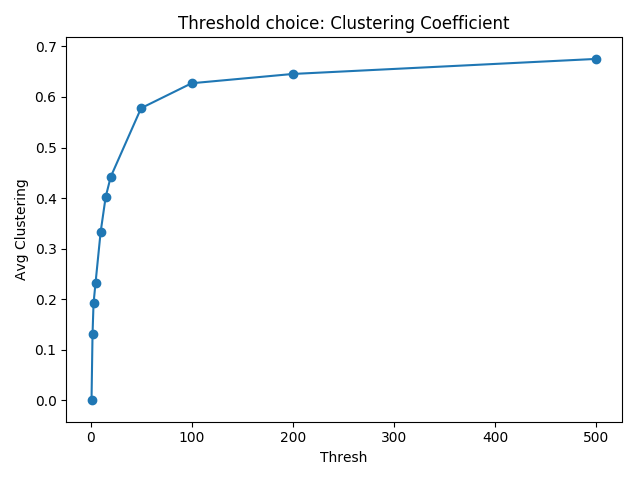
\includegraphics[width=1.\textwidth]{../data/plots/thresh_vs_avg_clustering.png}
        \caption{Clustering Coefficient vs. Threshold Size}
    \end{subfigure}
    ~
    \begin{subfigure}{0.4\textwidth}
        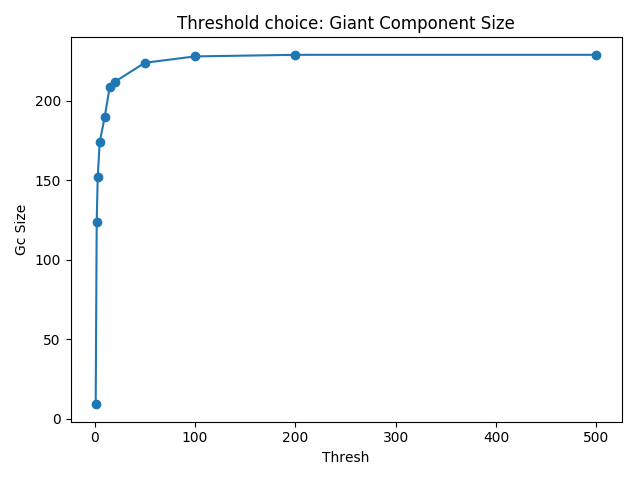
\includegraphics[width=1.\textwidth]{../data/plots/thresh_vs_gc_size.png}
        \caption{Giant Component Size vs. Threshold Size}
    \end{subfigure}
    \caption{Comparing threshold size effect on clustering coefficient and giant component size in order to determine the ideal threshold size.}
    \label{fig-threshold-size}
\end{figure*}

\subsubsection{Nodes and Edges}
Network nodes constitute each character identified in the set of found named entities. These were referenced against online resources to ensure proper coverage of the characters in the book. Edges in the book represent a co-mention between two entities in the text. A threshold number of tokens (words) under which the number of tokens between the mention of one entity and another determines if an edge is established. If the edge already exists, the weight is updated. The current entity $i$ is only matched with proceeding entities $j$ within this threshold. Once no match is found, the next available entity is checked for proceeding matches.

The threshold number of tokens is determined by a semi-objective measure of the effect of the threshold length on the average clustering coefficient and the giant component size (see Figure \ref{fig-threshold-size}). The intuition behind the use of these metrics is that we choose the minimum threhold length required to produce a large giant component and ample enough clustering best capturing the highly connected nature of characters in the novel. Our chosen threshold is 50 tokens.

